Systematic literature review was conducted to gain information about the current state of source code plagiarism study in academia. The database that was utilized to query research papers is called \emph{Scopus\footnote{\url{https://www.scopus.com/}}}, which is a web service containing peer-reviewed scientific literature. The service itself holds links to papers which are published under for example \emph{ACM (Association for Computing Machinery)} and \emph{IEEE (Institute of Electrical and Electronics Engineers)}, both of these being major computer science institutions. 

Following subchapters describe how the review was conducted and what kind of results were found. 

\subsection{Review process}

Querying Scopus can be done in a similar way as querying databases in SQL-like languages. The used query inside Scopus was following
\begin{verbatim}
TITLE-ABS-KEY (("plagiarism" OR "authorship identification")  
                AND "source code") 
AND  (LIMIT-TO (SUBJAREA,"COMP"))
\end{verbatim}

\noindent
This query translates to finding papers which title, abstract or keywords contains the word \emph{plagiarism} or \emph{authorship identification} and at least the term \emph{source code}. The reason to choose these keywords was to find papers which study the problem of plagiarism finding from source code either in general terms, or by utilizing authorship identification techniques. Next, the query limits the area of study to computer science to focus on plagiarism studies which utilize techniques found from computer science.

After the initial search, the goal of the second step was to limit the amount of papers. This was done by excluding all papers that were any of the following types: a review of certain aspect of source code plagiarism e.g. student motives behind plagiarism, an improvement to some pre-existing algorithm\footnote{In this context meaning algorithmic speedup}, plugin to online learning management systems, application to competition where the used method wasn't explained, study that used either byte-level information or information gathered during running the program, hashing techniques\footnote{Using the size of compression as a metric}, system review which didn't address the method and theses. 

Beside these attributes, included papers needed to also test their proposed method in some way and the amount of documents in experiment phase needed to be larger than two. The reason for including this as a limiting factor, was to gather studies that used test sets to evaluate the performance of their model in terms of accuracy, as this allows to compare used techniques more critically. 


\subsection{Review results}

The total number of papers gathered by querying Scopus in the first part of the literature review was 187, and the date when the query was done was 7th of February 2018. The distribution of paper per year can be seen in the following plot.

\begin{figure}[h]
\centering
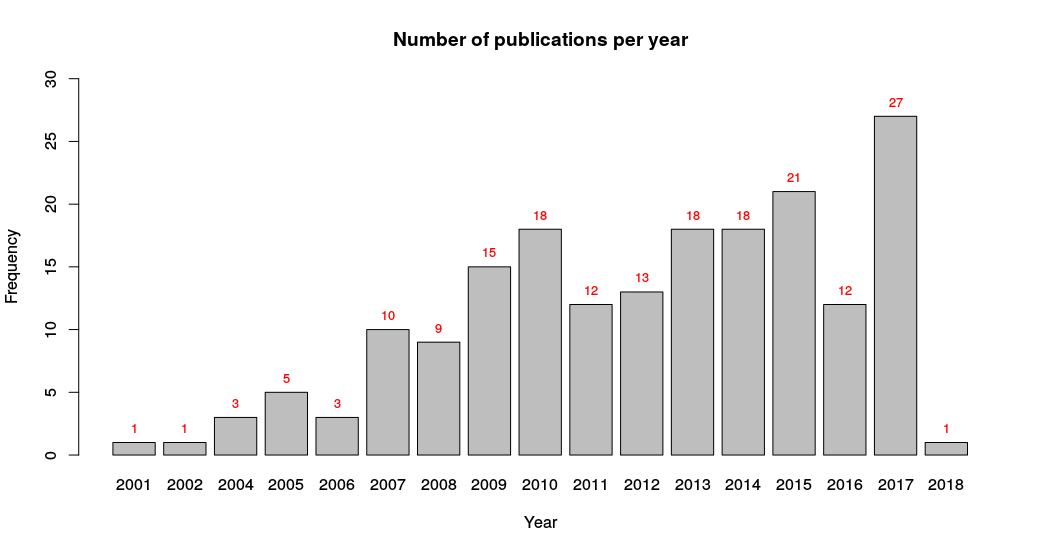
\includegraphics[width=\textwidth]{plots/Rplot.png}
\caption{Results of the first query to Scopus}
\end{figure}

\noindent
This set was filtered by terms described in the previous chapter, and the total number of papers inspected more carefully in this systematic literature review is 32. 

From the set of 32 studies, we look answers for following questions: \emph{how plagiarism can be detected from source code}, \emph{what are possible features that can be derived from source code} and \emph{how can one identify the author of a given source code}. We start first by grouping the papers by their themes to see what kind of different approaches there are to deal with the problem of plagiarism detection. After the initial classification, following aspects are identified from the studies: data, methods and test results. 


\subsubsection{Approaches}

The most high level division between papers could be done in a similar fashion as was used by the
query; dividing papers either to be about the detection of plagiarism or identifying the author of a given source code. However, during the literature review it was found that it's more clearer to make a division between similarity detection and identifying the authorship. This high-level division can be seen from the following table.

\begin{table}[ht]
    \caption{Papers divided into two high-level categories}
    \label{table-highcateq}
    \centering
    \begin{tabular}{ | c | c | }
        
        \hline
        {\bf Similarity detection} & {\bf Authorship identification} \\ \hline
    
        \cite{AFAPLI2015, LICD2010, AASCPD2012} & \cite{SCAANN2017, ABEC2014, CAPSCAP2014}   \\
        \cite{Heblikar2015NormalizationBS, USCR2014, AIR2015} &  \cite{SCANG2007, EJPFSAI2004, ACSBPD2012}\\
        \cite{OTIOLSS2015, BUAA2009, ramirez2015high} &  \cite{APASCAI2007, UCMHGAAI2007, ESHPFSCAC2008}\\
        \cite{Ohmann2015, TBCFPD2012, Fu2017WASTKAW} &  \cite{AIRTSCAA2009, TSUDIJSCAI2011, DNNSCAI2013} \\
        \cite{ASTMLPD2013, AAPSCDPTK2013, CPDPPD2013}    & \cite{SCAIUFL2013, SDNAIJSP2015, AISC2017} \\
        \cite{PACASCD2005, RCISCP2017} &  \\ \hline
        {\bf Number of papers} & {\bf Number of papers} \\ \hline
        17 & 15 \\ \hline
    \end{tabular}
\end{table}

\noindent
Even though papers divide quite evenly in table \ref{table-highcateq}, these high-level groups are still too large, and thus for the sake of clarity, we divide both into subgroups.

Similarity detection in itself can be further divided into at least two general categories based on the current tools \cite{RSCAD2016}: attribute and structure. Then naturally, as authorship identification uses features derived directly from the source code, we can use the same classification to authorship identification studies. However, based on the literature review, there are more finer categorizations that define the studies better based on the features they use, and thus we propose the following categories and their abbreviations: \emph{attribute counting (AC)}, \emph{segment matching (SM)}, \emph{n-gram (NG-STR)}, \emph{tree-based (AST-STR)} and lastly \emph{hybrid approaches (HYB-STR)}. If category has no studies under it, we leave the category out from the upcoming tables. These categories can be summarized briefly as following and are similar to categories identified from other similarity detection studies by Ali \etal \cite{OCPOCP2011}. 

\paragraph{Attribute counting}
Studies utilizing countable statistics, often referred as \emph{metrics}, that are gathered from source codes. This includes features like amount of words per line, number of lines per source code and number of keywords.

\paragraph{Segment matching}
Considers two source codes as two strings and finding maximum match between them i.e. longest common subsequence. These problems are also known as string matching problems, where one of the most famous algorithms is \emph{Greedy String Tiling} introduced early in \cite{SSGST1993}. We also categorize string similarity measures to this category like string edit distances.

\paragraph{$N$-gram}
Treating the source code as a string and splitting it via sliding window where the window size is the value of $n$ and the window traverses on either word or character level. This forms the vocabulary of the source code which is then transformed into occurrences of particular terms that are present, thus ultimately creating a vector representation of the source code. For example the statement \texttt{int a = 2} could be transformed into following word level 2-tuples using two as the value of $n$ (bigram). The first value of the following tuples is the $n$-gram extracted and the second value is the frequency: (\texttt{int a}, 1), (\texttt{a =}, 1), (\texttt{= 2}, 1). 

\paragraph{Tree-based methods}
Constructing a tree presentation from the source code, that captures the structure. The generation of a tree presentation usually requires some kind of parser because it's language specific feature. The inspection of a generated tree can be done via tree traversal methods for example using recursive functions. 

\paragraph{Hybrid methods}
Combine the usage of AST-structure with $n$-gram representation. For example it can be a method which traverses abstract syntax tree, prints it and generates $n$-gram representation from the output.
\\\\
The grouping of similarity detection papers can be seen from following table, where it's clear that most of the papers deal with similarity detection by utilizing structural features, indicated by the STR-ending, and many studies prefers to use $n$-gram representation of the source code.

\begin{table}[ht]
    \caption{Subgroups and sizes of similarity detection studies}
    \label{table-sdstudies}
    \centering
    \begin{tabular}{ | c | c | c | c | c |}
        
        \hline
        {\bf AC} & {\bf SM} & {\bf NG-STR} & {\bf AST-STR} & {\bf HYB-STR} \\ \hline
        \cite{PACASCD2005} & 
        \cite{LICD2010, ASTMLPD2013} & 
        \cite{AASCPD2012, USCR2014, AFAPLI2015} & 
        \cite{TBCFPD2012, AAPSCDPTK2013, AIR2015} & 
        \cite{BUAA2009, CPDPPD2013, RCISCP2017} \\
        & 
        & 
        \cite{Heblikar2015NormalizationBS, Ohmann2015, OTIOLSS2015} & 
        \cite{Fu2017WASTKAW} &
        \\
        & & \cite{ramirez2015high} &  & \\ \hline
        {\bf \#AC} & {\bf \#SM} & \multicolumn{3}{c |}{\bf \#STR} \\ \hline
        1 & 2 & \multicolumn{3}{c |}{14}
        \\ \hline
    \end{tabular}
\end{table}

When inspecting the division of authorship studies, we can see the division in table \ref{table-aistudies} is more evenly distributed contrast to similarity detection studies. More studies seems to utilize countable attributes from source codes and many also prefers to utilize $n$-grams, which is quite obvious when one considers that these methods are able to capture the writing style of an author from high-level features. For example authors can name the identifiers how they like, introduce comments and use various stylistic techniques when they write source code. 

\begin{table}[ht]
    \caption{Subgroups and sizes of authorship identification studies}
    \label{table-aistudies}
    \centering
    \begin{tabular}{ | c | c | c | c |}
        
        \hline
        {\bf AC} & {\bf NG-STR} & {\bf AST-STR} & {\bf HYB-STR} \\ \hline
        \cite{EJPFSAI2004, UCMHGAAI2007, APASCAI2007} & \cite{SCANG2007, ESHPFSCAC2008, AIRTSCAA2009} & \cite{SCAANN2017} & \cite{SDNAIJSP2015, AISC2017}\\ 
        \cite{ACSBPD2012, SCAIUFL2013, DNNSCAI2013} & \cite{TSUDIJSCAI2011, CAPSCAP2014, ABEC2014} & &\\ \hline
        {\bf \#AC} & \multicolumn{3}{c |}{\bf \#STR} \\ \hline
        6 & \multicolumn{3}{c |}{9}
        \\ \hline
    \end{tabular}
\end{table}

\newpage

Both of these results seems to show that utilizing structure is popular in both high-level classes, but quite dominant in similarity detection. However both groups of studies seems to show high popularity on $n$-gram methods, which is able to capture both individual style of the author and structural preferences. % source?
